%!TEX encoding = UTF-8 Unicode
%!TEX root = ../lect-w10.tex

%%%


\Subsection{Överskuggingsregler, \texttt{override}}

\begin{Slide}{Medlemmar, arv och överskuggning}\SlideFontTiny
\begin{multicols}{2}
\noindent Olika sorters överskuggningsbara medlemmar i \Emph{Scala}:
\begin{itemize}
\item \code{def}
\item \code{val}
\item \code{lazy val}
\item \code{var}
\end{itemize}

\columnbreak

\pause

\noindent Olika sorters överskuggningsbara instansmedlemmar i \Emph{Java}:
\begin{itemize}
\item variabel
\item metod
\end{itemize}

{\SlideFontTiny\noindent Medlemmar som är \jcode{static} kan ej överskuggas (men döljas) vid arv.}

\vspace{0.5em}
\end{multicols}

\pause
\begin{itemize}\SlideFontTiny
\item När man överskuggar \Eng{override} en medlemmen med en annan medlem med samma namn i en subtyp, får denna medlem en (ny) implementation.

\item Singelobjekt kan ej ärvas (och medlemmar i singelobjekt kan därmed ej överskuggas).

\item När man konstruerar ett objektorienterat språk gäller det att man definierar sunda överskuggningsregler vid arv. Detta är förvånansvärt knepigt.

\item Alla knepiga regler för överskuggning är svåra att lära sig utantill, men som tur är så hjälper kompilatorns felmeddelande dig att följa reglerna \code{:)}
\end{itemize}
\end{Slide}


\begin{Slide}{Fördjupning: Regler för överskuggning i Scala} \SlideFontTiny
\label{slideW07:overriderules}
En medlem M1 i en supertyp får överskuggas av en medlem M2 i en subtyp, enligt dessa regler: (se även \url{https://stackoverflow.com/questions/40057337})
\begin{enumerate}
\item M1 och M2 ska ha samma namn och typerna ska matcha.
\item \code{def} får bytas ut mot: \code{def}, \code{val}, och \code{lazy val}, och under speciella förutsättningar \code{var} (mer om att byta \code{def} mot \code{var} snart)
\item \code{val} får bytas ut mot \code{val}. Om medlemmen i M1 som överskuggas är abstrakt så får en \code{val} även bytas mot en \code{lazy val}.
\item En abstrakt \code{var} får bara bytas ut mot en \code{var}. En konkret \code{var} får ej bytas ut.
\item \code{lazy val} får bara bytas ut mot en \code{lazy val}.
\item Om en medlem i en supertyp är abstrakt \emph{behöver} man inte använda nyckelordet \code{override} i subtypen. (Men det är bra att göra det ändå så att kompilatorn hjälper dig att kolla att du verkligen överskuggar något.)
\item Om en medlem i en supertyp är konkret \emph{måste} man använda nyckelordet \code{override} i subtypen, annars ges kompileringsfel.
\item M1 får inte vara \code{final}.
\item M1 får inte vara \code{private}, men kan vara \code{private[X]} om M2 också är \code{private[X]}, eller \code{private[Y]} om X är (en del av) Y.
\item Om M1 är \code{protected} måste även M2 vara det.

\end{enumerate}
\end{Slide}

\begin{Slide}{Fördjupning: Överskugga \texttt{var} med \texttt{var}}\SlideFontTiny
Det krävs speciella förutsättningar för att överskugga en \code{var} med en \code{var}.
\begin{itemize}
\item En konkret medlem får \Alert{inte} bytas ut mot en \code{var} -- inte ens en konkret \code{var}:
\begin{REPLsmall}
scala> trait ConcreteVar { var x = 42 }
scala> trait Sub extends ConcreteVar { override var x = 43 }
-- Error:
1 |trait Sub extends ConcreteVar { override var x = 43 }
  |                                             ^
  |             error overriding variable x in trait ConcreteVar of type Int;
  |               variable x of type Int cannot override a mutable variable
\end{REPLsmall}
\item En abstrakt \code{var}-medlem får bytas ut mot en \code{var} om du \Alert{inte} skriver \code{override}:
\begin{REPLsmall}
scala> trait AbstractVar { var x: Int }
scala> trait Sub extends AbstractVar { override var x = 43 }
-- Error:
1 |trait Sub extends AbstractVar { override var x = 43 }
  |                                             ^
  |             error overriding variable x in trait AbstractVar of type Int;
  |               variable x of type Int cannot override a mutable variable
scala> trait Sub extends AbstractVar { var x = 43 }   // funkar utan override
// defined trait Sub
\end{REPLsmall}
\end{itemize}
Undvik abstrakta \code{var}-medlemmar -- oftast bättre med abstrakt \code{def}.
\end{Slide}

\begin{Slide}{Fördjupning: Överskugga \texttt{def} med \texttt{var}}\SlideFontTiny
\begin{itemize}
\item En abstrakt \code{def}-medlem får bytas ut mot en \code{var} om du \Alert{inte} skriver \code{override}:
\begin{REPLsmall}
scala> trait AbstractDef { def x: Int }
scala> trait Sub extends AbstractDef { override var x = 43 }
-- Error:
1 |trait Sub extends AbstractDef { override var x = 43 }
  |                                             ^
  |                                             setter x_= overrides nothing

scala> trait Sub extends AbstractVar { var x = 43 }   // funkar om ej override
\end{REPLsmall}
Den abstrakta \code{def}-medlemmen blir då implementerad av en konkret getter. 
\item Egentligen är en publik \code{var}-medlem en kombination av en getter och en setter. Du kan skapa konkret getter+setter och överskugga gettern explicit med \code{override} (notera att settern inte kan göra \code{override}, eftersom superklassen inte har någon motsvarande metod att byta ut -- jämför felmeddelande ovan):
\begin{REPLsmall}
scala> trait Sub2 extends AbstractDef:
         private var myPrivateValue = 42
         override def x: Int = myPrivateValue
         def x_(newValue: Int): Unit = myPrivateValue = newValue
\end{REPLsmall}
Ovan fungerar fint eftersom vi nu har en giltig kombination av getter+setter.
\end{itemize}
\end{Slide}


\Subsection{\texttt{super}}

\begin{Slide}{Att skilja på mitt och ditt med \texttt{super}}
\begin{REPL}
scala> class X { def gurka = "super pepino" }

scala> class Y extends X {
         override val gurka = ":("
         val sg = super.gurka
       }

scala> val y = new Y
y: Y = Y@26ba2a48

scala> y.gurka
res0: String = :(
\end{REPL}

\pause
Super Pepinos to the rescue:
\begin{REPLnonum}
scala> y.sg
res1: String = super pepino

\end{REPLnonum}


\pause
\begin{tikzpicture}[overlay]
\node at (7.5,1.7) {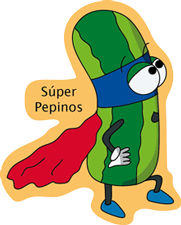
\includegraphics[scale=0.5]{../img/ttsuper}};
\end{tikzpicture}
\href{https://youtu.be/NPhjiXskz34}{\small https://youtu.be/NPhjiXskz34}
%\href{http://www.pepinadas.com/}{\small www.pepinadas.com/}
\end{Slide}



\begin{Slide}{Terminologi och nyckelord vid arv}

\SlideFontSize{7.5}{10}
\begin{tabular}{r  l}
\Emph{subtyp}           & en typ som ärver en supertyp\\
\Emph{supertyp}         & en typ som ärvs av en subtyp\\
\Emph{bastyp}           & en typ som är rot i ett arvsträd\\
\Emph{abstrakt medlem}  & en medlem som saknar implementation\\
\Emph{konkret medlem}   & en medlem som ej saknar implementation\\
\Emph{abstrakt typ}     & en typ som kan ha abstrakta medlemmar; kan ej instansieras\\
\Emph{konkret typ}      & en typ som ej har abstrakta medlemmar; kan instansieras\\
\code|class|            & en konkret typ som \Alert{kan ej ha abstrakta medlemmar}\\
\code|abstract class|   & en abstrakt typ som \Emph{kan ha abstrakta medlemmar}\\
\code|trait|            & är en abstrakt typ som \Emph{kan mixas in} \\
\code|extends|          & står före en supertyp, medför arv av supertypens medlemmar\\
\code|override|         & en medlem överskuggar (byter ut) en medlem i en superttyp\\
\code|protected|        & gör en medlem synlig i subtyper till denna typ (jmf \code|private|)\\
\code|final gurka|      & gör medlemen gurka final: förhindrar överskuggning\\
\code|final class|      & gör klassen final: förhindrar vidare subtypning\\
\code|sealed|           & förseglad trait/klass: enbart subtyper i denna kodfil, koll av match\\
\code|open class|       & berätta att den är tänkt att ärvas, \code|open| krävs för arv i annan kodfil\\   
\code|transparent trait|& gör typen osynlig vid typhärledning\\
\code|super.gurka|      & refererar till supertypens medlem \code|gurka| (jmf \code|this|)\\

\end{tabular}

\ifkompendium\else
\pause
\begin{tikzpicture}[overlay]
\node at (9.5,2) {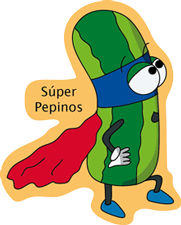
\includegraphics[scale=0.46]{../img/ttsuper}};
\end{tikzpicture}
\fi

\end{Slide}



\Subsection{Algebraiska datatyper}

\begin{Slide}{Terminologi för datatyper}\SlideFontSmall
\begin{itemize}
\item Abstrakt datatyp \Eng{abstract data type}
\begin{itemize}\SlideFontTiny
\item Definieras av gränssnittet och beteendet -- implementationen är dold för användaren. 
\item Fördelar: inkapsling, lokala ändringar, flexibilitet.
\item Skapas i Scala t.ex. med klasser + privata medlemmar.
\end{itemize} 
\item Enumeration, ä.k. uppräkning \Eng{enumeration}
\begin{itemize}\SlideFontTiny
\item En speciellt enkel form av s.k. algebraisk datatyp som består av en uppräknad, ändlig sekvens av enkla värden som har en ordning.
\item Skapas i Scala med 1) heltal, 2) \code{sealed trait} ... \code{case class} ... 3) \code{enum}
\end{itemize} 
\item Algebraisk datatyp \Eng{algebraic data type}, förk. ADT
\begin{itemize}\SlideFontTiny
\item En datatyp som är sammansatt av delar som kan kombineras. 
\item Två olika algebraiska datatyper som kan kombineras med varandra:
\begin{itemize}\SlideFontTiny
\item \Alert{Och}-typ (ä.k. produkt, record, struct), exempel: \\ \code|case class Person(namn: String, ålder: Int)| \\består av attributen namn \Alert{OCH} ålder.
\item \Emph{Eller}-typ (ä.k. summa, union), exempel: \code|enum Färg { case Röd, Svart}| \\kan vara antingen röd \Emph{ELLER} svart.
\end{itemize}  
\end{itemize} 
\end{itemize}
\end{Slide}

\begin{Slide}{En case-klass är en produkt.}
Klassen \code{Person} nedan har ett namn \Alert{och} en ålder.
\begin{REPL}
scala> case class Person(namn: String, ålder: Int)

scala> Person("Kim",42)
val res0: Person = Person(Kim,42)

scala> res0.isInstanceOf[Product]
val res1: Boolean = true

scala> res0.product   // Tryck TAB
productArity          productElement    productElementName
productElementNames   productIterator   productPrefix
          
scala> res0.productElementNames.toVector
val res2: Vector[String] = Vector(namn, ålder)

scala> res0.productElement
val res3: Int => Any = Lambda1981/0x00000008408f2840@44498af0

scala> res0.productElement(0)
val res4: Any = björn

\end{REPL} 
\end{Slide}


\begin{Slide}{Algebraisk datatyp, kombinerad produkt och summa}\SlideFontSmall
Med trait, case-klass och objekt:
\begin{Code}
sealed trait PersonId // summan av två subtyper (Number eller Missing)
object PersonId:  
  case class Number(n: Long) extends PersonId  // produkt med ett element
  case object Missing extends PersonId         // ett enkelt värde
\end{Code}
Motsvarande med \code{enum}:
\begin{Code}
enum PersonId:
  case Number(n: Long)
  case Missing     
\end{Code}
\begin{REPLsmall}
scala> Vector.tabulate(10)(i => 
         if i % 3 == 0 then PersonId.Missing else PersonNumber(i)
       )
val res0: Vector[Object] = Vector(Missing, PersonNumber(1), PersonNumber(2), Missing, 
  PersonNumber(4), PersonNumber(5), Missing, PersonNumber(7), PersonNumber(8), Missing)
\end{REPLsmall}

\end{Slide}

\begin{Slide}{Algebraisk datatyp med typparameter}\SlideFontSmall
Denna ADT har ett fall som är en \Emph{generisk} case-klass:     
\begin{Code}
sealed trait Kanske[+A]   // +A ger s.k. covarians, mer om det senare
object Kanske:
  case class Någon[A](a: A) extends Kanske[A]
  case object Ingen extends Kanske[Nothing]   
\end{Code}
Motsvarande med \code{enum}: (kompilatorn fyller i \code{extends ...} automatiskt)
\begin{Code}
enum Kanske[+A]:
  case Någon(a: A)
  case Ingen     
\end{Code}
Känner du igen denna? \pause Jämför inbyggda typen \code{Option}\\~\\Implementation av \code{getOrElse} med extensionsmetod, tips: använd \code{match} \pause
\begin{Code}
extension [A](k: Kanske[A]) def getOrElse(default: A):A = k match 
  case Kanske.Någon(a) => a
  case Kanske.Ingen => default
\end{Code}     
\end{Slide}

\begin{Slide}{Fördjupning: Typunioner med eller-operator}\SlideFontSmall
En mycket enkel summa-typ kan skapas med typ-operatorn \code{|} 
\begin{REPLsmall}
scala> var x: Int | String = 42
var x: Int | String = 42

scala> x = "hej" 
x: Int | String = hej

scala> type IntOrErr = Int | String
// defined alias type IntOrErr = Int | String

scala> def div(nom: Int, denom: Int): IntOrErr = 
         if denom != 0 then nom / denom else "div. by zero"
\end{REPLsmall}
Fördel jämfört med klass: rudimentärt enkelt.\\ Nackdelar: kan inte deklarera parametrar, medelemmar och allt annat som en klass kan; i viss mån kan detta kompensera med \code{extension} och \code{match}.\\ 
{\SlideFontTiny Läs mer här:
\url{https://dotty.epfl.ch/docs/reference/new-types/union-types.html}
}
\end{Slide}